\documentclass[12pt,a4paper,dvipdfmx]{jsarticle}
\usepackage[utf8]{inputenc}
\usepackage{amsmath,amsfonts,amssymb}
\usepackage{graphicx}
\usepackage{booktabs}
\usepackage{array}
\usepackage{longtable}
\usepackage{geometry}
\usepackage{fancyhdr}
\usepackage{caption}
\usepackage{subcaption}
\usepackage{float}
\usepackage{url}
\usepackage{hyperref}

% ページレイアウト設定
\geometry{left=25mm,right=25mm,top=30mm,bottom=30mm}

% ヘッダー・フッター設定
\pagestyle{fancy}
\fancyhf{}
\fancyhead[C]{ワイン品質予測における機械学習手法の比較研究}
\fancyfoot[C]{\thepage}

% キャプション設定
\captionsetup{font=small,labelfont=bf}

\title{ワイン品質予測における機械学習手法の比較研究\\
{\large ???}}
\author{学籍番号:\#\#\#\#\#\#\\
氏名:\#\#\#\#}
\date{2025年9月21日}

\begin{document}

\maketitle

\section{序論}

近年、機械学習技術の発展により、食品の品質評価における客観的な予測手法が注目されている。\cite{Yang2025}特に、ワインの品質評価は伝統的に専門家による官能評価に依存してきたが、理化学的な成分分析データから品質を予測することができれば、品質管理の効率化や客観性の向上が期待できる。

本研究の目的は、ワインの理化学的特性から品質を予測する回帰モデルの構築と評価である。具体的には、酸度、糖分、アルコール度数などの11の理化学的特徴量を用いて、3つの異なる機械学習手法(線形回帰、多層パーセプトロン、サポートベクター回帰)による品質予測性能を比較検討する。これにより、ワイン品質予測における各手法の特徴と有効性を明らかにし、実用的な品質予測システムの基盤となる知見を得ることを目指す。

\section{データと前処理}

\subsection{データセットの概要}

本研究では、UCI Machine Learning Repositoryで公開されているPortuguese "Vinho Verde" wine dataset\cite{Cortez2009}\cite{UCIWineQuality}の赤ワインデータを使用した。このデータセットは、ポルトガルの「ヴィーニョ・ヴェルデ」地域で生産された赤ワイン1,599本について、理化学的特性と品質評価を記録したものである。

データセットには以下の11個の特徴量が含まれている:

\begin{itemize}
    \item \textbf{固定酸度(fixed acidity)}: 主にタルタル酸などの不揮発性酸の濃度(g/dm³)
    \item \textbf{揮発性酸度(volatile acidity)}: 主に酢酸の濃度で、高すぎると不快な酢酸臭を生じる(g/dm³)
    \item \textbf{クエン酸(citric acid)}: 少量で酸味と清涼感を与える(g/dm³)
    \item \textbf{残留糖分(residual sugar)}: 発酵後に残った糖分の量(g/dm³)
    \item \textbf{塩化物(chlorides)}: 塩分濃度(g/dm³)
    \item \textbf{遊離亜硫酸(free sulfur dioxide)}: 微生物増殖と酸化を防ぐ(mg/dm³)
    \item \textbf{総亜硫酸(total sulfur dioxide)}: 遊離形と結合形の亜硫酸の総量(mg/dm³)
    \item \textbf{密度(density)}: ワインの密度(g/cm³)
    \item \textbf{pH}: 酸性度を示す指標(0-14スケール)
    \item \textbf{硫酸塩(sulphates)}: 抗酸化剤として使用される硫酸カリウム等(g/dm³)
    \item \textbf{アルコール度数(alcohol)}: エタノール含有量(\% vol)
\end{itemize}

目的変数である品質(quality)は、ワイン専門家による官能評価により0-10のスケールで評価されているが、実際のデータでは3-8の範囲に分布している。品質の分布を詳細に見ると、5と6の評価が最も多く、極端に良い(8)や悪い(3)評価は少数である。

\subsection{前処理手順}

データの前処理は以下の手順で実施した。

\textbf{データ分割}: 全データを学習用(70\%)、検証用(15\%)、テスト用(15\%)に分割した。具体的には、1,599本のワインを学習用1,119本、検証用240本、テスト用240本に分割した。この分割比率は、十分な学習データを確保しつつ、検証とテストで適切な評価を行うために設定した。

\textbf{学習・検証・テストデータの役割}: 学習データはモデルのパラメータを最適化するために使用し、検証データは学習中の早期終了判定とハイパーパラメータ調整に使用した。テストデータは最終的なモデル性能評価にのみ使用し、学習過程では一切使用しないことで、未知データに対する汎化性能を客観的に評価した。

\textbf{標準化処理}: 各特徴量は平均0、標準偏差1になるよう標準化を実施した。これは、特徴量間でスケールが大きく異なるため(例:pHは3-4の範囲、総亜硫酸は6-289の範囲)、学習の収束性を向上させ、各特徴量の寄与を公平に評価するために必要である。標準化は学習データの統計量を用いて実施し、検証・テストデータには同じ変換を適用した。

\section{手法}

\subsection{評価対象モデル}

本研究では、回帰問題における代表的な3つの手法を比較対象とした。

\subsubsection{線形回帰(Linear Regression)}

線形回帰は最も基本的な回帰手法であり、入力特徴量の線形結合により出力を予測する。数式で表すと、予測値$\hat{y}$は以下のように計算される:

\begin{equation}
\hat{y} = w_0 + w_1x_1 + w_2x_2 + \ldots + w_{11}x_{11}
\end{equation}

ここで、$w_i$は各特徴量の重み係数、$x_i$は標準化された特徴量、$w_0$はバイアス項である。

本実装では、PyTorchを用いてニューラルネットワーク形式で実装し、入力層から出力層への直接的な線形変換を行う。活性化関数は使用せず、純粋な線形回帰モデルとして構築した。重みの初期化には\textbf{Xavier uniform初期化}を採用した。Xavier uniform初期化は、各層の重みを$[-\sqrt{6/(n_{in} + n_{out})}, \sqrt{6/(n_{in} + n_{out})}]$の一様分布から初期化する手法で、$n_{in}$は入力次元数、$n_{out}$は出力次元数である。この初期化により、勾配の消失や爆発を防ぎ、安定した学習を実現した。

\subsubsection{多層パーセプトロン(MLP: Multi-Layer Perceptron)}

多層パーセプトロンは、複数の隠れ層を持つフィードフォワードニューラルネットワークである。各層の計算は以下の式で表される:

\begin{equation}
h^{(l+1)} = f(W^{(l)}h^{(l)} + b^{(l)})
\end{equation}

ここで、$h^{(l)}$は第$l$層の出力、$W^{(l)}$は重み行列、$b^{(l)}$はバイアスベクトル、$f$は活性化関数である。

本研究では、入力層(11次元)$\rightarrow$隠れ層1(128次元)$\rightarrow$隠れ層2(64次元)$\rightarrow$出力層(1次元)の4層構造を採用した。各隠れ層には\textbf{ReLU活性化関数}$f(x) = \max(0, x)$を適用し、非線形性を導入することで複雑なパターンの学習を可能にした。ReLUは勾配消失問題を軽減し、計算効率も高い利点がある。

過学習を抑制するため、各隠れ層後に\textbf{ドロップアウト層}を配置した。ドロップアウトは学習時にランダムにニューロンを無効化することで、モデルの汎化性能を向上させる正則化手法である。重みの初期化にはXavier uniform初期化を使用し、各層で適切な勾配の流れを確保した。

\subsubsection{サポートベクター回帰(SVR: Support Vector Regression)}

サポートベクター回帰は、サポートベクターマシンの回帰版であり、\textbf{$\varepsilon$-insensitive損失関数}を用いてロバストな予測を行う。$\varepsilon$-insensitive損失は以下のように定義される:

\begin{equation}
L_\varepsilon(y, f(x)) = \begin{cases} 
0 & \text{if } |y - f(x)| \leq \varepsilon \\
|y - f(x)| - \varepsilon & \text{otherwise}
\end{cases}
\end{equation}

この損失関数は、予測値と実測値の差が$\varepsilon$以下の場合は損失を0とし、それを超えた分のみをペナルティとして扱う。これにより、小さな誤差を許容し、外れ値に対してロバストな予測が可能となる。

SVRの最適化問題は以下の制約付き最適化問題として定式化される:

\begin{equation}
\min_{w,b,\xi,\xi^*} \frac{1}{2}||w||^2 + C\sum_{i=1}^n(\xi_i + \xi_i^*)
\end{equation}

ここで、$C$は正則化パラメータ、$\xi_i, \xi_i^*$はスラック変数である。本研究では、scikit-learnの実装を使用し、線形カーネルを採用した。SVRは外れ値に対してロバストな特性を持ち、高次元データにおいても効果的に動作することが知られている。

\subsection{ハイパーパラメータ調整とモデル学習}

各モデルについて、異なる最適化手法を用いてハイパーパラメータ調整を実施した。

\textbf{グリッドサーチ}は、事前に定義したハイパーパラメータの組み合わせを網羅的に評価する手法である。各組み合わせについて交差検証を行い、検証データでの性能が最も高い組み合わせを最適解として選択する。計算コストは高いが、定義された範囲内での最適解を確実に見つけることができる。

\textbf{SVRの最適化}: SVRでは、グリッドサーチによる系統的なハイパーパラメータ調整を実施した。SVRは非反復的なアルゴリズムであり、一度のトレーニングでモデルが完成するため、グリッドサーチが適している。

\textbf{PyTorchベースモデルの最適化}: 線形回帰とMLPでは、勾配降下法による反復学習を行った。各ハイパーパラメータ組み合わせについて、最大500エポックまで学習を行い、早期終了条件により最適な時点でのモデルを保存した。

\textbf{線形回帰のハイパーパラメータ}:
\begin{itemize}
    \item 学習率(learning rate): \{0.001, 0.005, 0.01, 0.02, 0.05\}
    \item ドロップアウト率(dropout rate): \{0.0, 0.05, 0.1, 0.2\}
    \item 重み減衰(weight decay): \{0.0, 0.001, 0.01\}
\end{itemize}

\textbf{MLPのハイパーパラメータ}:
\begin{itemize}
    \item 学習率: \{0.001, 0.002, 0.005, 0.01\}
    \item ドロップアウト率: \{0.0, 0.1, 0.2\}
    \item 重み減衰: \{0.001, 0.01, 0.1\}
    \item 隠れ層構造: (128, 64)で固定
\end{itemize}

\textbf{SVRのハイパーパラメータ}:
\begin{itemize}
    \item 正則化パラメータ(C): \{0.1, 1.0, 10.0, 100.0\}
    \item $\varepsilon$-tube parameter: \{0.01, 0.1, 0.2, 0.5\}
    \item カーネル係数(gamma): \{'scale', 'auto', 0.001, 0.01, 0.1, 1.0\}
\end{itemize}

gamma パラメータについて、'scale'は$\gamma = \frac{1}{n_{features} \times X.var()}$を意味し、特徴量数とデータの分散に基づいて自動調整される。'auto'は$\gamma = \frac{1}{n_{features}}$を意味し、特徴量数のみに基づく設定である。これらの自動設定により、データの特性に応じた適切なカーネル幅が選択される。

\subsection{学習設定}

\textbf{損失関数}: PyTorchベースのモデル(線形回帰、MLP)では平均二乗誤差(MSE)を損失関数として使用した。SVRでは標準的な$\varepsilon$-insensitive損失を使用した。

\textbf{最適化手法}: PyTorchベースのモデルではAdam最適化手法を採用した。Adamは適応的学習率を持ち、回帰問題において安定した収束性を示すことが知られている。

\textbf{早期終了条件}: 過学習を防ぐため、検証データのRMSEが20エポック連続で改善しない場合に学習を停止する早期終了を実装した。これにより、最適な汎化性能を示す時点でのモデル重みを保存した。

\textbf{バッチサイズ}: 全モデルでバッチサイズ64を使用した。これは、データセット規模と計算効率のバランスを考慮して設定した。

\subsection{評価手法}

モデルの性能評価には以下の3つの指標を使用した:

\textbf{平均平方根誤差(RMSE)}: 
\begin{equation}
    \text{RMSE} = \sqrt{\frac{1}{n} \sum_{i=1}^{n}(y_i - \hat{y}_i)^2}
\end{equation}
予測値と実測値の差の大きさを直感的に理解しやすい指標である。

\textbf{平均絶対誤差(MAE)}: 
\begin{equation}
    \text{MAE} = \frac{1}{n} \sum_{i=1}^{n}|y_i - \hat{y}_i|
\end{equation}
外れ値の影響を受けにくく、平均的な予測誤差を表す。

\textbf{決定係数($R^2$)}: 
\begin{equation}
    R^2 = 1 - \frac{\sum_{i=1}^{n}(y_i - \hat{y}_i)^2}{\sum_{i=1}^{n}(y_i - \bar{y})^2}
\end{equation}
モデルが目的変数の分散をどの程度説明できるかを示す。1に近いほど高い予測性能を意味する。

\subsection{実験手順}

実験は以下の手順で実施した:

\begin{enumerate}
    \item \textbf{データ前処理}: データ読み込み、分割、標準化を実行
    \item \textbf{ベースライン評価}: 各モデルのデフォルトパラメータでの性能を測定
    \item \textbf{ハイパーパラメータ調整}: 各パラメータを段階的に最適化
    \item \textbf{最終評価}: 最適パラメータでの学習・評価を実施
    \item \textbf{可視化}: 学習曲線、予測値散布図、残差分布を生成
\end{enumerate}

各実験において、学習過程の詳細な記録を取り、モデルの収束性や過学習の有無を確認した。

\section{結果}

\subsection{最終性能比較}

各モデルについて、ハイパーパラメータ調整過程で多数の組み合わせを評価したが、ここでは最適な組み合わせのみを報告する。各モデルの最適ハイパーパラメータでの性能を表\ref{tab:performance}に示す。

\begin{table}[h]
\centering
\caption{各モデルの性能比較}
\label{tab:performance}
\begin{tabular}{lcccc}
\toprule
モデル & Test RMSE & Test MAE & Test $R^2$ & 最適パラメータ \\
\midrule
MLP & \textbf{0.623} & 0.502 & \textbf{0.416} & lr=0.002, dropout=0.0, weight\_decay=0.01 \\
線形回帰 & 0.628 & \textbf{0.501} & 0.407 & lr=0.02, dropout=0.05, weight\_decay=0.0 \\
SVR & 0.631 & 0.516 & 0.400 & C=100.0, $\varepsilon$=0.1, gamma=scale \\
\bottomrule
\end{tabular}
\end{table}

MLPが最も優秀な性能を示し、Test RMSEで0.623、$R^2$で0.416を記録した。線形回帰は僅差で2位となり、Test RMSEで0.628を記録した。SVRは3位の結果となった。

\subsection{学習過程の分析}

\begin{figure}[H]
\centering
\includegraphics[width=0.7\textwidth]{../results/mlp/20250921_200150/figs/learning_curve.png}
\caption{MLP学習曲線: 訓練用RMSEと検証用RMSEの推移を示す。early stoppingにより適切な時点で学習が停止されている様子が確認できる。}
\label{fig:mlp_learning}
\end{figure}

\begin{figure}[H]
\centering
\includegraphics[width=0.7\textwidth]{../results/linear/20250921_213321/figs/learning_curve.png}
\caption{線形回帰学習曲線: trainとvalが極めて近い精度で収束する様子が観察される。}
\label{fig:linear_learning}
\end{figure}

図\ref{fig:mlp_learning}と図\ref{fig:linear_learning}に示すように、各モデルの学習過程を分析すると、MLPは約20-30エポックで最適な性能に達し、早期終了により過学習を適切に回避できた。線形回帰は約30-50エポックでの収束を示し、MLPよりもわずかに反復回数が上回った。

\subsection{予測精度の詳細分析}

\begin{figure}[H]
\centering
\includegraphics[width=0.6\textwidth]{../results/mlp/20250921_200150/figs/scatter_test.png}
\caption{予測値 vs 実測値散布図(MLP): MLPの予測値と実測値の関係を示す散布図。qualityが5~7の範囲で高い精度を示しているが、極端な品質値では予測誤差が大きくなる傾向が見られる。}
\label{fig:mlp_scatter}
\end{figure}

\begin{figure}[H]
\centering
\includegraphics[width=0.6\textwidth]{../results/linear/20250921_213321/figs/scatter_test.png}
\caption{予測値 vs 実測値散布図(線形回帰): 線形回帰の予測値と実測値の関係。MLPとほぼ同様の分布パターンを示している。}
\label{fig:linear_scatter}
\end{figure}

\begin{figure}[H]
\centering
\includegraphics[width=0.6\textwidth]{../results/svr/20250921_203231/figs/scatter_test.png}
\caption{予測値 vs 実測値散布図(SVR): SVRの予測値と実測値の関係。他の2手法と比較して,実測値とのばらつきがやや大きい。}
\label{fig:svr_scatter}
\end{figure}

図\ref{fig:mlp_scatter}、図\ref{fig:linear_scatter}、図\ref{fig:svr_scatter}の散布図分析により、全モデルが品質の中央値付近(5-6)での予測精度は高いが、極端な品質値(3-4、7-8)では予測精度が低下する傾向が確認された。これは訓練データにおける品質分布の偏りが影響していると考えられる。

\subsection{残差分析}

\begin{figure}[H]
\centering
\includegraphics[width=0.6\textwidth]{../results/mlp/20250921_200150/figs/residual_test.png}
\caption{残差分布ヒストグラム(MLP)}
\label{fig:mlp_residual}
\end{figure}

\begin{figure}[H]
\centering
\includegraphics[width=0.6\textwidth]{../results/linear/20250921_213321/figs/residual_test.png}
\caption{残差分布ヒストグラム(線形回帰)}
\label{fig:linear_residual}
\end{figure}

\begin{figure}[H]
\centering
\includegraphics[width=0.6\textwidth]{../results/svr/20250921_203231/figs/residual_test.png}
\caption{残差分布ヒストグラム(SVR)}
\label{fig:svr_residual}
\end{figure}

図\ref{fig:mlp_residual}、図\ref{fig:linear_residual}、図\ref{fig:svr_residual}の残差分析の結果、どの手法においても残差は概ね正規分布に従い、系統的なバイアスは確認されなかった。

\subsection{ハイパーパラメータ感度分析}

各モデルにおけるハイパーパラメータの影響を分析した結果、以下の知見が得られた:

\textbf{MLPにおける知見}:
\begin{itemize}
    \item 学習率0.002が最適であり、より高い学習率では不安定な学習となった
    \item ドロップアウト率0.0が最適で、この問題設定では正則化効果よりも表現力の保持が重要であった
    \item 重み減衰0.01が適切な正則化効果を提供した
\end{itemize}

\textbf{線形回帰における知見}:
\begin{itemize}
    \item 学習率0.02が最適で、MLPより高い学習率が必要であった
    \item ドロップアウト率0.05で若干の性能向上が見られた
    \item 重み減衰の効果は限定的であった
\end{itemize}

\textbf{SVRにおける知見}:
\begin{itemize}
    \item 線形カーネルが最適で、この問題は本質的に線形性が強いことが示唆された
    \item 正則化パラメータCは大きな値(100)が適していた
    \item $\varepsilon$-tubeは0.1のときに適切なバランスとなった
\end{itemize}

\section{考察}

\subsection{モデル間の比較と特徴}

実験結果から、3つのモデルは予想以上に類似した性能を示した。最も優秀なMLPと3位のSVRの間でも、Test RMSEの差は0.008(約1.3\%)に過ぎない。これは、ワイン品質予測問題における特徴量と目的変数の関係が比較的単純で、線形に近い構造を持つことを示唆している。

MLPが最高性能を示した理由として、適度な非線形性により特徴量間の相互作用を捉えることができた点が挙げられる。しかし、その優位性は僅かであり、計算コストや解釈性を考慮すると、線形回帰も実用的な選択肢として十分である。

線形回帰がMLPに次いで優れるという結果は、ワインの理化学的特性と品質の関係が主に線形であることを示している。

SVRの性能が他の2手法に比べてやや劣った理由として、データの線形性が高いため、SVRの主要な利点である非線形マッピングや外れ値ロバスト性が十分に発揮されなかった可能性がある。ただし、SVRは学習時間が短く、ハイパーパラメータ調整が比較的容易である利点がある。

\subsection{モデルの限界と課題}

今回の実験において、いくつかの限界と課題が明らかになった。

\textbf{予測範囲の制約}: 全モデルが品質スコアの極値(3-4、7-8)において予測精度が低下する傾向を示した。これは訓練データにおける品質分布の偏りに起因しており、品質5-6のサンプルが全体の約80\%を占めることが影響している。実用的な品質予測システムでは、この問題への対策が必要である。


\textbf{汎化性能の評価}: 本研究は単一の地域(ポルトガル・ヴィーニョヴェルデ)のワインデータに基づいており、他の地域や品種への汎化性能は未検証である。より広範囲なデータでの検証が必要である。

\textbf{非線形関係の探索}: MLPが僅かながら最高性能を示したものの、より複雑な非線形関係を捉えるための手法(例:決定木系手法、深層学習)の検討余地がある。


\section{結論}

本研究では、ワインの理化学的特性から品質を予測する回帰問題において、線形回帰、多層パーセプトロン、サポートベクター回帰の3手法を比較検討した。

実験の結果、以下の主要な知見が得られた:

第一に、MLPが最も優秀な性能(Test RMSE: 0.623, $R^2$: 0.416)を示したものの、線形回帰も僅差(Test RMSE: 0.628, $R^2$: 0.407)で続いた。この結果は、ワイン品質予測問題における特徴量と目的変数の関係が主に線形であることを示している。

第二に、適切なハイパーパラメータ調整により、比較的単純な線形回帰でも高い予測性能を達成できることが確認された。これは、計算コストや解釈性を重視する実用的なシステムにおいて重要な示唆である。

第三に、全モデルに共通して、品質の極値における予測精度の低下が観察された。これは訓練データの品質分布の偏りに起因しており、実用化に向けては、データ拡張や重み付き学習などの手法による改善が必要である。

第四に、SVRは他の2手法にやや劣る結果となったが、これはデータの線形性が高いことが原因と考えられる。より複雑で非線形な関係を持つデータセットでは、SVRの優位性が発揮される可能性がある。

本実験で得られた知見は、食品品質予測における機械学習手法の選択指針として有用である。特に、問題の複雑さに応じた適切な手法選択の重要性が示された。線形的な関係が支配的な問題では、解釈性と計算効率に優れる線形手法が実用的であり、複雑な非線形関係が予想される場合にのみ、より高度な手法を検討すべきである。

本研究を通じて、これまで主に画像の分類問題に取り組んできた私にとって、回帰問題を扱うことができたのは大きな経験となった。誤差を定量的に捉え、数値予測の難しさと面白さを実感できたことは、今後の研究活動においても重要な糧となる。本実験で得られた知見や視点を、自身の研究テーマにも応用し、より汎用的かつ実践的な成果へとつなげていきたい。

\section*{付録: 実験環境}

\begin{itemize}
    \item Python 3.11, PyTorch, scikit-learn, pandas, numpy
    \item 計算環境: CPU環境での実行
    \item 実験実行日: 2025年9月21日
\end{itemize}


\begin{thebibliography}{9}

\bibitem{Yang2025}
X.\ Yang, L.\ Zhu, W.\ Jiang, Y.\ Yang, L.\ Niu, Y.\ Zhao, Y.\ Wang, L.\ Chen, M.\ Gan, L.\ Zhu, and L.\ Shen,  
“Artificial intelligence-driven food quality prediction: Applying machine learning ensemble models for dynamic forecasting of pork pH and meat color changes,”  
\emph{Food Chemistry}, vol.\ 492, Part 2, 145383, Nov.\ 2025.  
Available: \url{https://doi.org/10.1016/j.foodchem.2025.145383}

\bibitem{Cortez2009}
P.\ Cortez, A.\ Cerdeira, F.\ Almeida, T.\ Matos, and J.\ Reis,
“Modeling Wine Preferences by Data Mining from Physicochemical Properties,”
\emph{Decision Support Systems}, vol.\ 47, no.\ 4, pp.\ 547–553, 2009.

\bibitem{UCIWineQuality}
P.\ Cortez, A.\ Cerdeira, F.\ Almeida, T.\ Matos, and J.\ Reis,
\emph{Wine Quality [Dataset]}, UCI Machine Learning Repository, 2009.
Available: \url{https://archive.ics.uci.edu/ml/datasets/Wine+Quality}

\end{thebibliography}

\end{document}